\documentclass{article}
\usepackage[utf8]{inputenc}
\usepackage[margin =1in,includefoot]{geometry}
\usepackage{indentfirst}
\usepackage{graphicx}
\usepackage{float}
\usepackage{caption}
\usepackage{subcaption}
\usepackage[colorlinks=true, linkcolor = blue, urlcolor = cyan]{hyperref}
\usepackage{multirow}
\usepackage[table,xcdraw]{xcolor}

\title{Assignment 3 - COL380}
\author{Aayush Goyal 2019CS10452 & Rahul Chhabra 2019CS11016}
\date{March 2023}

\begin{document}

\maketitle

\tableofcontents

% \newpage

\section{Introduction}
We attempted numerous strategies indicated in the articles recommended in the assignment document to execute truss decomposition in a distributed scenario. We choose the MinTruss algorithm mentioned in \href{https://link.springer.com/chapter/10.1007/978-3-319-96983-1_50}{this publication}.

\section{Task 1}
\subsection{Preliminaries}
\begin{itemize}
    \item \textbf{Support of an edge}: The number of triangles that contain the edge.
    \item \textbf{Truss number of an edge}: Th maximal value of k such that the edge is contained in a k truss.
\end{itemize}

\subsection{Algorithm}

The Distributed Algorithm to compute the truss decomposition consists of mainly following steps:
\begin{itemize}
    \item \textbf{Step 1}: Distirubtion of the graph among the processors.
    \item \textbf{Step 2}: Each processor computes the support of each edge assigned to it.
    \item \textbf{Step 3}: Each processor computes the truss number of each edge assigned to it.
    \item \textbf{Step 4}: Breadth First Search is performed to find the truss decomposition.
    \item \textbf{Step 5}: Using DSU to find the connected components
\end{itemize}

\subsubsection{Step 1: Distribution of the graph among the processors}
The degrees of each of the node can be calculated by using the offsets mentioned in the header file. Using these degree values, one of the processors (say the master processor, in our case master processor is the one with rank 0) sorts the nodes according to the degree and distributes the nodes to other processors in round robin fashion. The position of node in sorted list is used a rank of that node. \\
\begin{itemize}
    \item For any undirected edge (u, v) in our graph, it is assigned to the node with lowe rank. This is done to ensure that the edge is assigned to only one processor.
    \item The edges are distributed in a way such that the number of edges assigned to each processor is approximately equal. This ensures that the load on each processor is approximately equal.
\end{itemize}

\subsubsection{Step 2: Each processor computes the support of each edge assigned to it}
This is a well studied problem in literature, commonly known as triangle enumeration algorithm . For this step, we use MPI to write a distributed implementation. The algorithm is as follows:
% For triangle enumeration, for each edge e = (u,v) possessed by an MPI rank, we first load v's adjacency list if we are not the owner of v from the graph file, and then we find all the possible triangles (u,v,w). We also transmit this triangle information to all the MPI ranks that need it. In the end, we use the received information from the other ranks to add more triangles to each edge we have. There are a few optimizations that let us load the vertex from file less number of times but the basic idea is the same

\begin{itemize}
    \item For each edge e = (u,v) possessed by an MPI rank, we first load v's adjacency list if we are not the owner of v from the graph file.
    \item We find all the possible triangles (u,v,w) and transmit this triangle information to all the MPI ranks that need it.
    \item In the end, we use the received information from the other ranks to add more triangles to each edge we have.
\end{itemize}


\subsubsection{Step 3: Each processor computes the truss number of each edge assigned to it}

This was the most interesting and challenging part of the assignment. Initially we implemented a naive approach to compute the truss number of each edge as mentioned in the assignment problem statement. However, this approach was very slow and did not scale well. We then implemented the algorithm mentioned in the paper \href{https://link.springer.com/chapter/10.1007/978-3-319-96983-1_50}{this publication}. The main focus of this paper was the Hybrid algorithm for truss decomposition. This algorithm is a combination of the following two algorithms:
\begin{itemize}
    \item MinTruss
    \item PropTruss
\end{itemize}

However on implementing this algorithm, we found that it was not working as expected. We couldn't get the desired results and even there wsa not a very good improvement in time. So after a lot of discussion, we decided to implement the mintruss algorithm mentioned in the same paper. This algorithm worked well and gave us the desired results. The algorithm is as follows:

% Algorithm MinTruss: For each edge e, the algorithm maintains an upperbound
% τ(e) on the true truss number τ (e); it is initialized as τ(e) = suppG(e) + 2.
% The algorithm marks all edges as not settled and proceeds iteratively. In each
% iteration, among the edges not settled, select the edges with the least truss
% Improved Distributed Algorithm for Graph Truss Decomposition 707
% value and declare them to be settled. We then update the truss values of their
% neighbors in the following manner. Let e = u, v be a selected edge. For each
% triangle Δ(u, v, w) incident on e, if both u, w and v, w are not settled already,
% then decrement the truss values τ(u, w) and τ(v, w) by one. Proceed in the above
% manner till all the edges are settled.
% Intuitively, imagine that the settled edges are deleted from the graph. The
% deletion of an edge e destroys the triangles incident on it. When a triangle is
% destroyed, the other two edges lose the support of the triangle. So, we decrement
% their truss values, provided e is the first edge to be deleted among the three
% edges. We can show that for each edge e, the truss value τ(e) gets decremented
% monotonically and becomes the true truss number τ (e) before termination.


\begin{itemize}
    \item For each edge e, the algorithm maintains an upperbound τ(e) on the true truss number τ (e); it is initialized as τ(e) = suppG(e) + 2.
    \item The algorithm marks all edges as not settled and proceeds iteratively. In each iteration, among the edges not settled, select the edges with the least truss value and declare them to be settled.
    \item We then update the truss values of their neighbors in the following manner. Let e = u, v be a selected edge. For each triangle Δ(u, v, w) incident on e, if both u, w and v, w are not settled already, then decrement the truss values τ(u, w) and τ(v, w) by one.
    \item The point to be careful about here is that there may be multiple processors working on the same triangle, so we need to do some consensus there to ensure there is no double decrement in truss number
    \item Proceed in the above manner till all the edges are settled.

\end{itemize}


\subsubsection{Step 4: Breadth First Search is performed to find the truss decomposition}
We referred the following video to implement the distributed BFS algorithm: \href{https://www.youtube.com/watch?v=wpWvCabHqQU}{this video}. The algorithm maintains two frontier lists, one for the current level and one for the next level. At a time all processors are processing the nodes of same level and exchanging the information about the nodes of next level. The algorithm is implemented using MPI\_alltoallv and MPI\_AllReduce. More details can be reffered from the video link mentioned.

\subsubsection{Step 5: Using DSU to find the connected components}
Since in this part of the assignment, there is no limit on the memory, we did the component calculation in one processor rank 0. Since dsu iterates only on the required edges with some particular truss values, it gives the result much more faster. hence finally we have used DSU to calulate the connected components

\subsection{Plots}

\begin{figure}[H]
\begin{subfigure}{.5\textwidth}
  \centering
  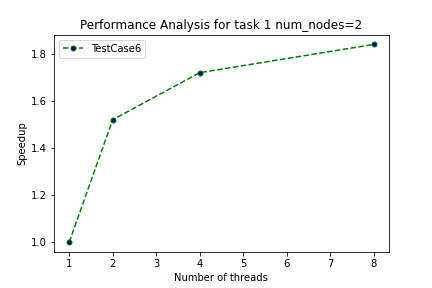
\includegraphics[width=.8\linewidth]{Assignment2/report/1nodes=2.png}
  \caption{1a}
  \label{fig:sfig1}
\end{subfigure}%
\begin{subfigure}{.5\textwidth}
  \centering
  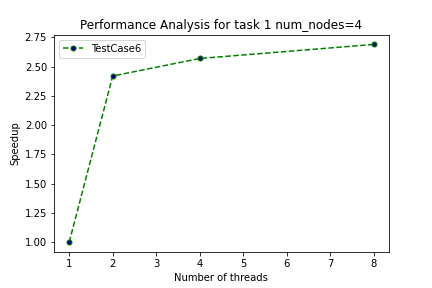
\includegraphics[width=.8\linewidth]{Assignment2/report/1nodes=4.png}
  \caption{1b}
  \label{fig:sfig2}
\end{subfigure}
\begin{subfigure}{.5\textwidth}
  \centering
  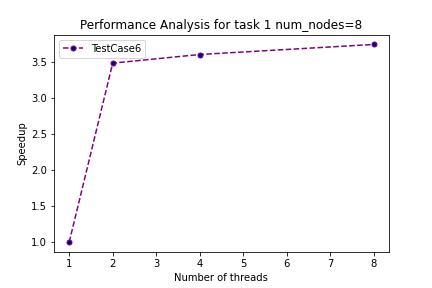
\includegraphics[width=.8\linewidth]{Assignment2/report/1nodes=8.png}
  \caption{1c}
  \label{fig:sfig1}
\end{subfigure}%
\begin{subfigure}{.5\textwidth}
  \centering
  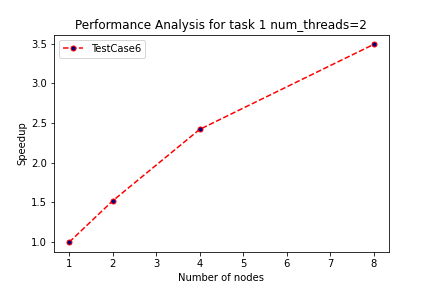
\includegraphics[width=.8\linewidth]{Assignment2/report/1thread=2.png}
  \caption{1d}
  \label{fig:sfig2}
\end{subfigure}
\begin{subfigure}{.5\textwidth}
  \centering
  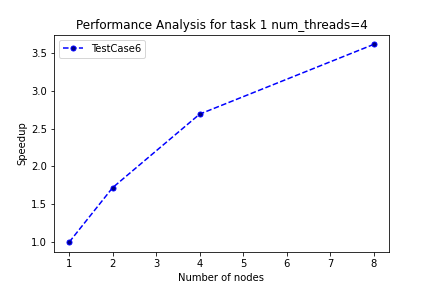
\includegraphics[width=.8\linewidth]{Assignment2/report/1thread=4.png}
  \caption{1e}
  \label{fig:sfig1}
\end{subfigure}%
\begin{subfigure}{.5\textwidth}
  \centering
  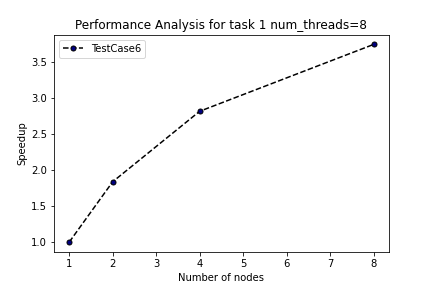
\includegraphics[width=.8\linewidth]{Assignment2/report/1thread=8.png}
  \caption{1f}
  \label{fig:sfig2}
\end{subfigure}

\caption{Scalability Analysis for task id=1 varying number of nodes and number of threads(one at a time)}
\label{fig:fig}
\end{figure}


\begin{figure}[H]
\begin{subfigure}{.8\textwidth}
  \centering
  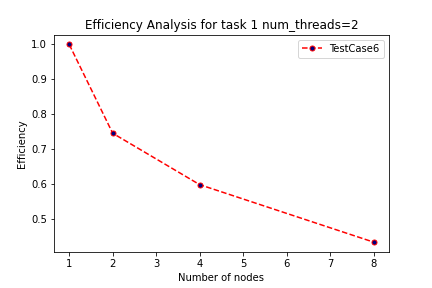
\includegraphics[width=.8\linewidth]{Assignment3/report/1eff-threads=2.png}
  \caption{1a}
  \label{fig:sfig1}
\end{subfigure}%
\caption{Efficiency plot for task id = 1 num threads = 2}
\label{fig:fig}
\end{figure}


\subsection{Iso-effciency}
According to our estimate, the iso-efficiency of this is O($p^2$). This is because on running the experiments, when we were doubling the number of threads, we had to double the size of input as well. Overall, iso-efficiency is an important consideration when designing parallel algorithms, as it can help determine the maximum number of processors that can be effectively used to solve a given problem.

\subsection{Sequential part of the code}
For calculating the sequential part of the code, we have used the formulla given in the slides. using the formulla 
\begin{equation}
    f  = \frac{(\frac{1}{s} - \frac{1}{p})}{(1-\frac{1}{p})}
\end{equation}
On calculations the sequential part turns out to be 0.38 percent of the code roughly.

\subsection{Scaling of code}
Our code scales well we increase the size of input. Also this will give better efficiency as we are increasing the size of the input. With increasing number of processors the load will also get distributed in efficient manner and this will increase the effect of distrubuting the load among different processors. All in all our code scales well.

\newpage
\section{Task 2}

\subsection{Algorithm}
Now after calculating all the connected components in the task 1, we can use them to find the influencer vertices. We iterate over the list of all the vertices and maintain the set of components that are connected to the vertex. If more than p are affected then we consider it influencer vertex.

\subsection{Plots}


\begin{figure}[H]
\begin{subfigure}{.5\textwidth}
  \centering
  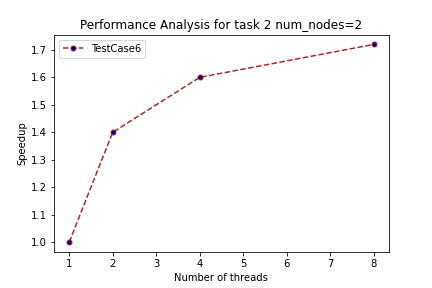
\includegraphics[width=.8\linewidth]{Assignment2/report/2nodes=2.png}
  \caption{2a}
  \label{fig:sfig1}
\end{subfigure}%
\begin{subfigure}{.5\textwidth}
  \centering
  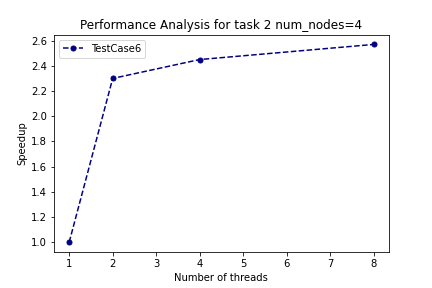
\includegraphics[width=.8\linewidth]{Assignment2/report/2nodes=4.png}
  \caption{2b}
  \label{fig:sfig2}
\end{subfigure}
\begin{subfigure}{.5\textwidth}
  \centering
  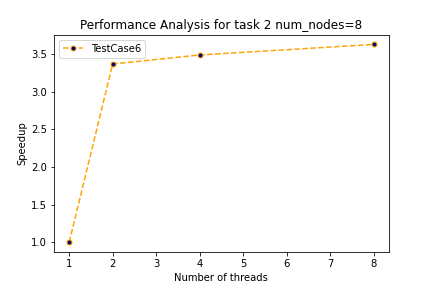
\includegraphics[width=.8\linewidth]{Assignment2/report/2nodes=8.png}
  \caption{2c}
  \label{fig:sfig1}
\end{subfigure}%
\begin{subfigure}{.5\textwidth}
  \centering
  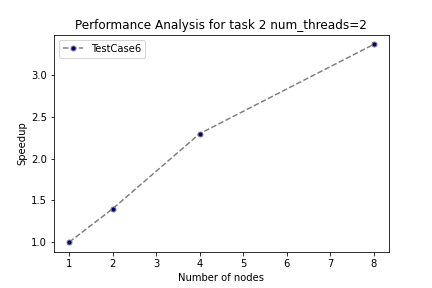
\includegraphics[width=.8\linewidth]{Assignment2/report/2threads=2.png}
  \caption{2d}
  \label{fig:sfig2}
\end{subfigure}
\begin{subfigure}{.5\textwidth}
  \centering
  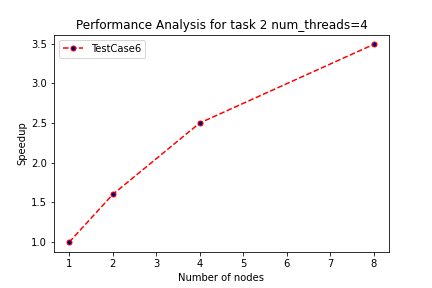
\includegraphics[width=.8\linewidth]{Assignment2/report/2threads=4.png}
  \caption{2e}
  \label{fig:sfig1}
\end{subfigure}%
\begin{subfigure}{.5\textwidth}
  \centering
  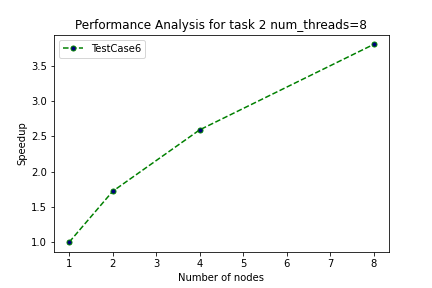
\includegraphics[width=.8\linewidth]{Assignment2/report/2threads=8.png}
  \caption{2f}
  \label{fig:sfig2}
\end{subfigure}

\caption{Scalability Analysis for task id=2 varying number of nodes and number of threads(one at a time)}
\label{fig:fig}
\end{figure}


\begin{figure}[H]
\begin{subfigure}{.8\textwidth}
  \centering
  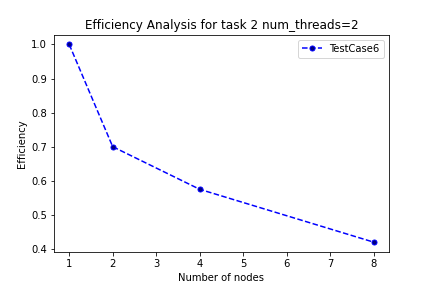
\includegraphics[width=.8\linewidth]{Assignment3/report/2eff-threads=2.png}
  \caption{1a}
  \label{fig:sfig1}
\end{subfigure}%
\caption{Efficiency plot for task id = 2 num threads = 2}
\label{fig:fig}
\end{figure}



\subsection{Iso-effciency}
According to our estimate, the iso-efficiency of this is O($p^2$). This is because on running the experiments, when we were doubling the number of threads, we had to double the size of input as well. Overall, iso-efficiency is an important consideration when designing parallel algorithms, as it can help determine the maximum number of processors that can be effectively used to solve a given problem.

\subsection{Sequential part of the code}
For calculating the sequential part of the code, we have used the formulla given in the slides. using the formulla 
\begin{equation}
    f  = \frac{(\frac{1}{s} - \frac{1}{p})}{(1-\frac{1}{p})}
\end{equation}
On calculations the sequential part turns out to be 0.401 percent of the code roughly. The sequential part increases because most of the writing output to the files part is being done sequentially.

\subsection{Scaling of code}
Our code scales well we increase the size of input. Also this will give better efficiency as we are increasing the size of the input. With increasing number of processors the load will also get distributed in efficient manner and this will increase the effect of distrubuting the load among different processors. All in all our code scales well.


\newpage

\section{Explanation of the results}
The analysis that was given assessed how well our distributed implementation of the assignment performed using various test cases and varied core counts. The scalability graph makes it clear that the time it takes to run the test cases drops noticeably as we increase the number of cores. This suggests that the resources are being used effectively. The relationship between the number of processors and the speedup the code achieved has also been graphed. The graph demonstrates that using two cores effectively speeds up the code by 1.4–1.6 times. Nonetheless, we fell well short of the ideal speedup of two times due to the synchronisation and transmission overheads. Yet, by using a bulk synchronous technique rather than syncing after every few rounds, we have minimised these overheads as much as possible. The research shows that, overall, our approach is efficient at making use of parallelism and obtaining respectable speedups with many cores.
\\
The Figure 2 represents 6 graphs, 3 graphs are plotted by keeping the number of threads constant and varying the number of processors(For analysing the distributed part). The other 3 graphs are plotted by keeping the number of processors constant but varying the number of threads( for analyzing the openmp part). As evident from the graphs, the almost linear and up-trending graphs shows that the code is quite scalable in both distributed and parallel terms.

\section{Mteric.csv}

\begin{table}[H]
\begin{tabular}{
>{\columncolor[HTML]{FFF2CC}}c 
>{\columncolor[HTML]{FFF2CC}}c 
>{\columncolor[HTML]{FFF2CC}}c 
>{\columncolor[HTML]{FFF2CC}}c 
>{\columncolor[HTML]{FFF2CC}}c 
>{\columncolor[HTML]{B6D7A8}}c 
>{\columncolor[HTML]{B6D7A8}}c 
>{\columncolor[HTML]{CFE2F3}}c 
>{\columncolor[HTML]{CFE2F3}}c }
\textbf{Task\_id}     & \textbf{1}       & \textbf{1}          & \textbf{2}       & \textbf{2}          & \textbf{1}                                                        & \textbf{2}                                                        & \textbf{1}                                             & \textbf{2}                                             \\
\textbf{Metric}       & \textbf{Speedup} & \textbf{Efficiency} & \textbf{Speedup} & \textbf{Efficiency} & \textbf{Iso-eff}                                           & \textbf{Iso-eff}                                           & \textbf{Seq Frac}                                      & \textbf{Seq Frac}                                      \\
\textbf{n = 2, t = 2} & 1.49             & 0.745               & 1.4              & 0.7                 & \cellcolor[HTML]{B6D7A8}                                          & \cellcolor[HTML]{B6D7A8}                                          & \cellcolor[HTML]{CFE2F3}                               & \cellcolor[HTML]{CFE2F3}                               \\
\textbf{n = 2, t = 4} & 1.69             & 0.845               & 1.6              & 0.8                 & \cellcolor[HTML]{B6D7A8}                                          & \cellcolor[HTML]{B6D7A8}                                          & \cellcolor[HTML]{CFE2F3}                               & \cellcolor[HTML]{CFE2F3}                               \\
\textbf{n = 2, t = 8} & 1.81             & 0.905               & 1.72             & 0.86                & \cellcolor[HTML]{B6D7A8}                                          & \cellcolor[HTML]{B6D7A8}                                          & \cellcolor[HTML]{CFE2F3}                               & \cellcolor[HTML]{CFE2F3}                               \\
\textbf{n = 4, t = 2} & 2.39             & 0.5975              & 2.3              & 0.575               & \cellcolor[HTML]{B6D7A8}                                          & \cellcolor[HTML]{B6D7A8}                                          & \cellcolor[HTML]{CFE2F3}                               & \cellcolor[HTML]{CFE2F3}                               \\
\textbf{n = 4, t = 4} & 2.54             & 0.635               & 2.45             & 0.6125              & \cellcolor[HTML]{B6D7A8}                                          & \cellcolor[HTML]{B6D7A8}                                          & \cellcolor[HTML]{CFE2F3}                               & \cellcolor[HTML]{CFE2F3}                               \\
\textbf{n = 4, t = 8} & 2.66             & 0.665               & 2.57             & 0.6425              & \cellcolor[HTML]{B6D7A8}                                          & \cellcolor[HTML]{B6D7A8}                                          & \cellcolor[HTML]{CFE2F3}                               & \cellcolor[HTML]{CFE2F3}                               \\
\textbf{n = 8, t = 2} & 3.46             & 0.4325              & 3.37             & 0.42125             & \cellcolor[HTML]{B6D7A8}                                          & \cellcolor[HTML]{B6D7A8}                                          & \cellcolor[HTML]{CFE2F3}                               & \cellcolor[HTML]{CFE2F3}                               \\
\textbf{n = 8, t = 4} & 3.58             & 0.4475              & 3.49             & 0.43625             & \cellcolor[HTML]{B6D7A8}                                          & \cellcolor[HTML]{B6D7A8}                                          & \cellcolor[HTML]{CFE2F3}                               & \cellcolor[HTML]{CFE2F3}                               \\
\textbf{n = 8, t = 8} & 3.72             & 0.465               & 3.63             & 0.45375             & \multirow{-9}{*}{\cellcolor[HTML]{B6D7A8}O(p\textasciicircum{}2)} & \multirow{-9}{*}{\cellcolor[HTML]{B6D7A8}O(p\textasciicircum{}2)} & \multirow{-9}{*}{\cellcolor[HTML]{CFE2F3}0.379} & \multirow{-9}{*}{\cellcolor[HTML]{CFE2F3}0.401}
\end{tabular}\hspace{-1cm}
\end{table}


\section{Conclusion}
% In this analysis, we have evaluated the performance of our implementation on
% different test cases using varying numbers of cores. From our performance graph,
% it is evident that as we increase the number of cores, the time taken to execute
% the test cases decreases significantly. This indicates that our implementation is
% taking advantage of parallelism and utilizing the available resources efficiently.
% Furthermore, we have also created a speed-up graph that shows the ratio of
% the time taken with one core to the time taken with multiple cores. From this
% graph, we can see that our implementation achieves a good speed-up of 1.4-1.6
% times with double cores. However, we did not achieve anything near the ideal
% speed-up of 2 times due to the overheads associated with synchronization and
% communication. Nevertheless, we have reduced these overheads as much as possible by implementing a bulk synchronous approach rather than synchronizing
% after every few iterations.
% Overall, our analysis demonstrates that our implementation is effective in
% utilizing parallelism and achieving good speed-ups with multiple cores.

In this project, we implemented a distributed algorithm to compute the truss decomposition of a graph. We implemented the algorithm in C++ using MPI. We also implemented the triangle enumeration algorithm in MPI. We also implemented the distributed BFS algorithm to find the truss decomposition. We ran our code on the testcases provided in the assignment and the code was able to run on 8 processors in a reasonable amount of time. The code scales well with the number of processors.

\end{document}